\documentclass{article}
\usepackage[dvips,a3paper,landscape,centering,margin=2cm]{geometry}
\usepackage{multicol}
\usepackage[utf8]{inputenc}
\usepackage{color}
\usepackage{amsmath}
\usepackage{graphicx}  
\definecolor{azulillo}{rgb}{0.8,0.85,1}
\definecolor{marronrp3}{rgb}{.9,.9,.7}
\definecolor{salmon}{rgb}{1,.9,.8}
\definecolor{rojo}{rgb}{.6,.1,0}
\pagestyle{empty}
\def\to{\rightarrow}
\hyphenation{coa-gu-la-tion frag-men-ta-tion}
\title{}
\author{}
\date{}

\begin{document}
	\begin{center}
		\begin{minipage}{.96\linewidth}
			\begin{center}
				\Huge \textbf{Euler's Constant to 1271 Places}
			\end{center}
		\end{minipage}
		
		\begin{minipage}{.5\linewidth}
			\begin{center}
				\vspace{.5cm}
				\emph{\textbf{By Donald E.Knuth}}
			\end{center}
		\end{minipage}
	\end{center}
	\vspace{.1cm}
	
	\setlength{\columnsep}{1cm}
	\begin{multicols}{3}
		\noindent
		\colorbox{salmon}{
			\begin{minipage}[t]{.96\linewidth}
				\vspace{.05cm}
				\begin{center}
					\vspace{.2cm}
					\section*{\Huge Main result}
					\Large The value of Euler's or Mascheroni's constant \\
					$\gamma$  =  $\lim_{n\to\infty}$ ̣(1+$\frac{1}{2}+...+\frac{1}{n}-\ln{n}$) 
				\end{center}
				
				\Large It is defined as the limiting difference between the harmonic series and the natural logarithm and is now determined to 1271 decimal places based on using  as Euler's summation formula. In addition, we still use Determination of Partial Quotients in order to find best rational approximations to $\gamma$, we represent it as a continued fraction. 
				\vspace{.1cm}
			\end{minipage}
		}
		\vspace{-0.5cm}
		\section*{Historical Background}
		\begin{minipage}[t]{.96\linewidth}
                \vspace{-0.5cm}  
			\Large At that time, Euler's constant was frist evaluated by Leonhard Euler, and he obtained the value 0.577218 in 1735. By 1781 he had calculated it more exactly as 0.5772156649015325. The calculations were carried out more precisely by several later mathematicians, among them Gauss, who obtained
			\begin{center}
				$\gamma$ = 0.577215664901532860606.    
			\end{center}
			\Large Adams' result stood until 1952, when Wrench found 328 decimal places.
			Although much work has been done trying to decide whether $\gamma$ is  rational or not? The
			evaluation has not been carried out any more precisely. With the use of high-speed
			computers, the constants $\pi$ and $\epsilon$ have been accurately evaluated to many thousands of decimal places. The evaluation of $\gamma$ to many places is considerably more difficult.
		\end{minipage}


            \vspace{-0.3cm}
		\section*{Evalution of $\gamma$}
            \vspace{-0.3cm}
		\Large We use Euler's summation formula in the form
		\begin{equation*}
			\hspace{-3cm} \sum_{i=1}^{n} f(i) = \int_{1}^{n} f(x)dx + \frac{1}{2}(f(n)+f(1))
		\end{equation*}
		\begin{equation*}
			\hspace{2cm}+\sum_{j=1}^{k} \frac{B_2j}{(2j)!} [f^{(2j-1)}(n)-f^{(2j-1)}(1)]  + R_k
		\end{equation*}
		
		\noindent
		\colorbox{marronrp3}{
			\begin{minipage}[t]{.96\linewidth}
				\vspace{.2cm}
				\vspace{.05cm}
				$R_k$: Remainder\\
				$B_m$: Bernoulli\hspace{0.1cm} Numbers\\
				$f^{(2j-1)}(n)$: (2j-1) \hspace{0.1cm}Derivative\hspace{0.1cm} at \hspace{0.1cm} (n)\\
				$\to The \hspace{0.1cm} purpose\hspace{0.1cm} is\hspace{0.1cm} to\hspace{0.1cm} assign\hspace{0.1cm}value\hspace{0.1cm} to\hspace{0.1cm} string\hspace{0.1cm} \sum_{i=1}^{n} f(i)$
				\hspace{.05cm}\
			\end{minipage}
		}
		\noindent
		\begin{minipage}[t]{.96\linewidth}
			\vspace{.3cm}
			\begin{itemize}
				\Large\item  $B_m$ are defined symbolically by $e^{B_x} = \frac{x}{e^x-1}$
			\end{itemize} \\
		\end{minipage}
		
		\noindent
		\begin{minipage}[t]{.96\linewidth}
			\vspace{.3cm}
			\begin{itemize}
				\Large \item$R_k$ is given by
			\end{itemize} \\
			\begin{equation*}
				R_k = \frac{1}{(2k+1)!} \int_{1}^{n} P_{2k+1} (x) f^{(2k+1)} (x)dx
			\end{equation*}
		\end{minipage}
		\begin{minipage}[t]{.96\linewidth}
			\vspace{.3cm}
			\begin{itemize}
				\Large \item $P_{2k+1} (x)$ is a periodic Bernoulli polynomial 
			\end{itemize}
			\begin{equation*}
                \hspace{-0.2cm}
				P_{2k+1}(x)={(\{x\}+B)}^{2k+1}={(-1)}^{k-1}(2k+1)!\sum_{r=1}^\infty \frac{2sin(2r{\pi}x)}{(2r{\pi})^{2k+1}}
			\end{equation*}
			\Large where \{x\} is the fractional part of x
		\end{minipage}
		
		\noindent
		\begin{minipage}[t]{.96\linewidth}
			\vspace{.3cm}
			\begin{itemize}
				\Large\item Periodic Bernoulli polynomial level 2k+1
			\end{itemize} \\
			
			\begin{center}
    		   $|P_{2k+1} (x)| \leq \frac{2(2k+1)!}{(2\pi)^{2k+1}}\sum_{r=1}^{\infty}\frac{1}{r^{2k+1}}$
			\end{center}
			
		\end{minipage}
		
		\noindent
		\begin{minipage}[t]{.96\linewidth}
			\vspace{.3cm}
			\begin{itemize}
				\Large\item The range of values of $\int_n^\infty \frac{P_{2k+1} (x)}{x^{2k+2}}$
			\end{itemize} \\
			\begin{equation*}
				\bigg|\int_n^\infty \frac{P_{2k+1} (x)dx}{x^{2k+2}}\bigg| \leq \frac{4}{n}\sqrt{\frac{k}{\pi}}(\frac{k}{n\pi{e}})^{2k}
			\end{equation*}
		\end{minipage}
		
		
		
		
		% ---------------------------------------------------------------------------
		 \vspace{-0.5cm}
		\section*{Determination of Partial Quotients}
            \vspace{-0.5cm}
            \begin{minipage}[t]{.96\linewidth}
                \Large This formula found best rational approximations to $\gamma$
            \end{minipage}
            
		\begin{minipage}[t]{.96\linewidth}
			    \centering
			    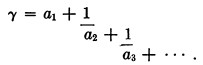
\includegraphics[scale=0.9]{p.jpg}
			    \label{fig:my_label}
		\end{minipage}

            \begin{minipage}[t]{.96\linewidth}
                \vspace{-0.5cm}\Large \hspace{-0.5cm}Matrix representation of the sequence $P_i, Q_i$
            \end{minipage}
             \begin{equation*}
             \left(
            \begin{array}{cc}
                    P_{i+1} & P_i  \\
                    Q_{i+1} & Q_i 
            \end{array}
            \right)=
            \left(
            \begin{array}{cc}
                    a_1 & 1  \\
                    1 & 0 
            \end{array}
            \right)
            \left(
            \begin{array}{cc}
                    a_2 & 1  \\
                    1 & 0 
            \end{array}
            \right)...
            \left(
            \begin{array}{cc}
                    a_i & 1  \\
                    1 & 0 
            \end{array}
            \right)
            \end{equation*}  

            \hspace{-0.5cm}\Large Formula determine Khintchine's constant applies to all real numbers with a partial quotients, where K $\approx$ 2.685 
            \begin{equation*}
                \lim \sqrt[n]{a_2a_3...a_{n+1}}=K
            \end{equation*}

            \hspace{-0.5cm}\Large Formula determine $\gamma$ but don't need Bernoulli numbers to avoid the bottleneck, which was used by Dura W.Sweenet to calculate 3566 decimal digits
            \vspace{-0.3cm}
            \begin{equation*}
                \gamma + \ln{n} = \sum_{k=1}^{\infty} \frac{(-1)^{k-1}n^k}{k!k} - \int_n^\infty\frac{e^{-x}}{x}dx
            \end{equation*}
            



            \vspace{-1cm}
		\section*{Details of Illustrative Example}
            \vspace{-0.5cm}
            \colorbox{marronrp3}{
                \begin{minipage}[t]{.96\linewidth}
                \Large We use method of Knopp to determine $\gamma$		      \begin{equation*}
		        \gamma=1+\frac{1}{2}+...+\frac{1}{n}-\ln{n}-\frac{1}      {2n}+\frac{B_2}{2n^2}+...+\frac{B_{2k}}{2kn^{2k}}
		      \end{equation*}
                \begin{equation*}
                    \hspace{7.5cm}
                     -\int_n^{\infty} \frac{P_{2k+1}(x)}{x^{2k+2}}dx
                \end{equation*}
                \end{minipage}
            }

            \hspace{-0.5cm}\Large   Step 1: Determine sum of $S_{1000} = 1+\frac{1}{2}+...+\frac{1}{1000}$\\
            \vspace{-0.8cm}
            \begin{itemize}
                \item Combine two adjacent terms to reduce the number of times division is performed
                
                \vspace{-0.2cm}\item $S_{10000}=(1+\frac{1}{2})+(\frac{1}{3}+\frac{1}{4})+...+(\frac{1}{9999}+\frac{1}{10000})=9.787606036...$
            \end{itemize}
            \vspace{-0.2cm}
            \Large Step 2: Determine $\ln{(10000)}$\\
            \vspace{-0.8cm}
            \begin{itemize}
                \item Find small values of $(x,y,z)$ so that $x+y\log_2{3}+\log_2{5}$ $\approx$ 0. We find (-1,5,-3),(-4,4,-1) and (6,5,-6)
                \vspace{-0.2cm}\item Find the numbers a, b, c so that $(2^{-1}3^55^{-3})^a.(2^{-4}3^45^{-1})^b.(2^63^55^{-6})^c=10000$. After calculating, we get a=-292, b=200, c=92 
                \vspace{-0.2cm}\item Finally, we have $\ln{(10000)}=-292\ln{(1-0.028)}+200\ln{(1+0.0125)}+92\ln{(1-0.004672)}$
            \end{itemize}
            \hspace{-0.3cm}
            \colorbox{marronrp3}{
                \begin{minipage}[t]{.98\linewidth}
                    
            \Large Step 3: Find sum expressions of Bernoulli numbers\\
            \vspace{-1cm}
            \begin{itemize}
                \item $B_{2k}^{'}=10^{-8k}{B_{2k}}$ were evaluated using the recursion
                
                \vspace{-0.6cm}
                \begin{equation*}
                            \left(
                            \begin{array}{cc}
                                2k+1 \\2k  
                            \end{array}
                            \right)B_{2k}^{'} +10^{-8}
                            \left(
                            \begin{array}{cc}
                                2k+1 \\2k-2  
                            \end{array}
                            \right)B_{2k-2}^{'}+...+   
                \end{equation*}
                \begin{equation*}
                \vspace{-0.06cm}
                     \hspace{3.5cm}
                            10^{8-8k}\left(
                            \begin{array}{cc}
                                2k+1 \\2  
                            \end{array}
                            \right)B_2^{'} =\frac{2k-1}{2.10^{8k}}
                \end{equation*}
            \end{itemize}
            
            \begin{itemize}
                \item\Large $S=\frac{B_2}{2n^2}+\frac{B_4}{4n^4}+...+\frac{B_250}{250n^250}$
            \end{itemize}
                \end{minipage}
            }
            
            \vspace{0.3cm}\hspace{-0.5cm}\Large Step 4: Combine all values in steps, give the result of $\gamma$	
	\end{multicols}
	
\end{document}
